\chapter{Case Study}
\label{ch:case_study}

%\newcommand{\mysubparagraph}[1]{\subparagraph{#1}\mbox{}\\}

\lettrine[lines=4, loversize=-0.1, lraise=0.1]{T}{his} chapter consists of two parts. In the first part an effort is made to check how much complete are the tools in measuring agility compared to one another. In the second part, this study aims to check the correlation of the practices covered by \ac{PAM}, \ac{TAA} and \ac{OPS} by performing a case study in company F.

\section{Research Purpose}
The purpose of this study is to analyse if three agility measurement tools correlate with each other and see if they assess agility in similar ways. In addition, it analyses how complete are one to another.

\newcounter{tmpc} % set the counter to continue the RQs

\subsection{Research Questions}
\begin{enumerate}
	\item How much complete are the tools in measuring agility?
	\item In what ways do the tools correlate?
	\setcounter{tmpc}{\theenumi} % set the counter to continue the RQs
\end{enumerate}



\section{Tools Completeness}
\label{sec:tools_completeness}

\subsection[\ac{TAA} Areas]{Team Agility Assessment Areas}
Team Agility Assessment (\ac{TAA}) does not claim that it covers specific agile practices, but rather areas important for a team. It focuses on product ownership for Scrum teams but also on the release and iteration planning and tracking. The team factor plays a great role, as well as the development practices and the working environment. Automated testing is important here as well. Finally, it is worth mentioning that it is the only tool focusing so much on the release planning. In Table~\ref{table:taa_practices} one can see \ac{TAA}'s areas.

\begin{table}
  \begin{tabular}{| p{5cm} p{5cm} |}
    \hline
    \multicolumn{2}{|c|}{\textbf{\ac{TAA} Areas}}  \\ \hline
     \begin{itemize} \item Product Ownership \item Release Planning and Tracking \item Iteration Planning and Tracking \end{itemize} &
     \begin{itemize}  \item Team \item Testing Practices \item Development Practices / Infrastructure \end{itemize}  \\ \hline
  \end{tabular}
  \captionof{table}{Areas covered by \ac{TAA}}
  \label{table:taa_practices}
\end{table}

\subsection[\ac{PAM} Practices]{Perceptive Agile Measurement Practices}
The Perceptive Agile Measurement (\ac{PAM}) tool focuses on the iterations during software development but also on the stand-up meetings among the team members, their collocation and the retrospectives they have. The customers access and their acceptance criteria have a high significance as well. Finally, the continuous integration and the automated unit testing are considered crucial in order to be agile. In Table~\ref{table:pam_practices} one can see \ac{PAM}'s practices.

\begin{table} [H]
  \begin{tabular}{| p{6cm} p{6cm} |}
    \hline
    \multicolumn{2}{|c|}{\textbf{\ac{PAM} Practices}}  \\ \hline
    	\begin{itemize} \item Iteration Planning \item Iterative Development \item Continuous Integration and Testing \item Co-Location \end{itemize} &
     \begin{itemize} \item Stand-up Meetings \item Customer Access \item Customer Acceptance Tests \item Retrospectives \end{itemize}  \\ \hline
  \end{tabular}
  \captionof{table}{Agile practices covered by \ac{PAM}}
  \label{table:pam_practices}
\end{table}

\subsubsection[\ac{OPS} Practices]{Objectives, Principles, Strategies Practices}
Objectives, Principles, Strategies (\ac{OPS}) Framework is the successor of the Objectives, Principles, Practices (\ac{OPP}) Framework \cite{opp}. \ac{OPP} identified 27 practices as implementations of the principles which later on were transformed into 17 strategies. In Table~\ref{table:opp_practices} one can see \ac{OPP}'s practices. 

\begin{table}
\begin{tabular}{| p{7.5cm}  p{7.5cm} |}
	\hline
	\multicolumn{2}{|c|}{\textbf{\ac{OPP} Practices}}  \\ \hline
     	\begin{itemize}
     		\item Iterative and Incremental Development 
     		\item Continuous Feedback 
     		\item Evolutionary Requirements 
     		\item Smaller and Frequent Product Releases 
     		\item Customer/User Acceptance Testing 
     		\item Frequent Face-to-Face Communication
     		\item Refactoring 
     		\item Automated Test Builds
     		\item Software Configuration Management 
     		\item Test Driven Development
     		\item Iteration Progress Tracking and Reporting 
     		\item Code Ownership 
     		\item Retrospectives Meetings 
     		\item Just-in-Time Refinement of Features /Stories/Tasks 
     	\end{itemize} 
     	& \begin{itemize}
     	 	\item Appropriate Distribution of Expertise
  			\item Self-Organizing Teams
     		\item Client-Driven Iterations 
     		\item Product Backlog 
     		\item Agile Project Estimation 
     		\item Adherence to Coding Standards 
     		\item Physical Setup Reflecting Agile Philosophy
     		\item Daily Progress Tracking Meetings 
     		\item Minimal or Just Enough Documentation 
     		\item Minimal Big Requirements Up Front and Big Design Up Front 
     		\item Collocated Customers
     		\item Constant Velocity 
     		\item Pair Programming  
 		\end{itemize} 
     \\ \hline
\end{tabular}
\captionof{table}{Agile practices covered by \ac{OPP}}
\label{table:opp_practices}
\end{table}

\subsubsection[Tool Practices]{Practices Covered Between The Tools}

As it can be clearly seen in Tables~\ref{table:opp_practices}, \ref{table:pam_practices} and \ref{table:taa_practices}, the \ac{OPP}, and as a consequence the \ac{OPS}, covers more agile practices than the other tools. \\

In the next pages a mapping between \ac{OPP} and \ac{PAM} (see Table~\ref{table:opp_pam_practices}) and \ac{OPP} and \ac{TAA} (see Table~\ref{table:opp_taa_practices}) follows. \\

Some of the \ac{OPP} practices though have abstracted to \ac{OPS} strategies in order to avoid repetition of the questions' mapping and to better reflect the \ac{OPS} Framework. The \ac{OPP} practices 
\begin{inparaenum} [a\upshape)]
	\item \textit{Frequent Face-to-Face Communication},
	\item \textit{Physical Setup Reflecting Agile Philosophy}, and
	\item \textit{Collocated Customers}
\end{inparaenum} have been abstracted to the \ac{OPS} strategy \textit{High-Bandwidth Communication}  \cite[p. 57]{sventha_dissertation}. In the same way, the \ac{OPP} \textit{Automated test builds} practice has been abstracted to the \ac{OPS} strategy \textit{Continuous Integration} \cite[p. 57]{sventha_dissertation}. \\

The connection between the practices and strategies is done based on the questions of each tool. The aforementioned connections are depicted with colours. When a practice has more than one colour, it is because it covers more practices from the other tool (The colours and symbols among Tables~\ref{table:opp_pam_practices}, ~\ref{table:opp_taa_practices} are randomly selected and do not imply any connection between the two tables). \\

\begin{table}
\begin{tabular}{| p{6.8cm} | p{8cm} |}
	\hline
	\textbf{\ac{PAM}} & \textbf{\ac{OPP}/\ac{OPS}}  \\ \hline
		 \begin{itemize}[leftmargin=*, label=]
 			\item {\color{RoyalBlue1}Iteration Planning} \FourStar
 			\item {\color{DarkMagenta}Iterative Development} \JackStarBold
 			\item {\color{DarkOrange1}Continuous Integration and Testing} \AsteriskRoundedEnds 
 			\item {\color{DeepPink1}Co-Location} \Asterisk 
 			\item {\color{green4}Stand-up Meetings} \EightStar
 			\item {\color{DarkBlue}Customer Access} \JackStar
 			\item {\color{red2}Customer Acceptance Tests} \AsteriskThin
 			\item {\color{DarkRed}Retrospectives} \CrossMaltese
 		\end{itemize}
 		&
     	\begin{itemize}[leftmargin=*, label=]
     		\item {\color{RoyalBlue1}Iteration Progress Tracking and Reporting} \FourStar
     		\item {\color{RoyalBlue1}Iterative} {\color{DarkMagenta}and Incremental  Development} \FourStar ~\JackStarBold
     		\item {\color{DarkOrange1}Continuous Integration} \AsteriskRoundedEnds
     		\item {\color{DarkOrange1}Software Configuration Management} \AsteriskRoundedEnds
     		\item {\color{DarkOrange1}Test Driven} {\color{red2}Development} \AsteriskRoundedEnds ~\AsteriskThin 
     		\item {\color{DarkBlue}High-Bandwidth} {\color{DeepPink1}Communication} \JackStar ~\Asterisk 
     		\item {\color{green4}Daily Progress Tracking Meetings} \EightStar
     		\item {\color{DarkBlue}Client-Driven} {\color{RoyalBlue1}Iterations} \JackStar ~\FourStar
     		\item {\color{red2}Evolutionary Requirements} \AsteriskThin
     		\item {\color{red2}Customer/User Acceptance Testing} \AsteriskThin
     		\item {\color{DarkRed}Retrospectives Meetings} \CrossMaltese
     		\item {\color{RoyalBlue1}Self-Organizing Teams} \FourStar
 		\end{itemize} 
     \\ \hline
\end{tabular}
\caption{Relation of \ac{OPP}/\ac{OPS} and \ac{PAM} practices}
\label{table:opp_pam_practices}
\end{table}

\begin{table}
\begin{tabular}{| p{7cm} | p{7.8cm} |}
	\hline
	\textbf{\ac{TAA}} & \textbf{\ac{OPP}/\ac{OPS}}  \\ \hline
		\begin{itemize}[leftmargin=*, label=] 
     		\item {\color{DeepPink1}Product Ownership} \Asterisk 
     		\item {\color{green4}Release Planning and Tracking} \EightStar
     		\item {\color{RoyalBlue1}Iteration Planning and Tracking} \FourStar
     		\item {\color{DarkRed}Team} \CrossMaltese
     		\item {\color{DarkOrange1}Testing Practices} \AsteriskRoundedEnds
     		\item {\color{DarkMagenta}Development Practices/Infrastructure} \JackStar	
 		\end{itemize} 
		&	
     	\begin{itemize}[leftmargin=*, label=]
     		\item {\color{DeepPink1} Iterative and Incremental Development} \Asterisk 
     	    \item {\color{DeepPink1}Product Backlog} \Asterisk 
     		\item {\color{green4}Smaller and Frequent Product Releases} \EightStar
     		\item {\color{RoyalBlue1}Customer/User {\color{green4}Acceptance Testing}} \FourStar ~\EightStar
     		\item {\color{RoyalBlue1}Constant Velocity} \FourStar	
     		\item {\color{RoyalBlue1}Iteration Progress Tracking and Reporting} \FourStar
     		\item {\color{DarkRed}Self-} {\color{green4}Orga}{\color{RoyalBlue1}nizing} {\color{DarkMagenta}Teams} \CrossMaltese ~\EightStar ~\FourStar ~\JackStar 
     		\item {\color{DarkRed}Appropriate Distribution of Expertise} \CrossMaltese
     		\item {\color{DarkRed}High-Bandwidth Communication} \CrossMaltese 
     		\item {\color{DarkRed}Daily Progress Tracking Meetings} \CrossMaltese
     		\item {\color{DarkRed}Retro}{\color{RoyalBlue1}spectives} {\color{green4}Meetings}  \CrossMaltese ~\FourStar ~\EightStar 
     		\item {\color{DarkOrange1}Test Driven Development} \AsteriskRoundedEnds
     		\item {\color{DarkMagenta}Refactoring} \JackStar
     		\item {\color{DarkMagenta}Software Configuration Management} \JackStar
     		\item {\color{DarkMagenta}Adherence to Coding Standards} \JackStar
     		\item {\color{DarkMagenta}Pair Programming} \JackStar
     		\item {\color{DarkMagenta}Continuous} {\color{DarkOrange1}Integration} \JackStar ~\AsteriskRoundedEnds
     	\end{itemize} 
     \\ \hline
\end{tabular}
\caption{Relation of \ac{OPP}/\ac{OPS} and \ac{TAA} practices/areas}
\label{table:opp_taa_practices}
\end{table}


\subsubsection[\ac{PAM} and \ac{TAA} Mapping]{Mapping of questions from the \ac{PAM} and \ac{TAA} tools}
\label{mapping}

\ac{PAM} has divided its questions based on agile practices, while on the other hand, the \ac{TAA} has divided them based on areas considered important. In the next pages, there is a mapping between the questions used from the \ac{PAM} and \ac{TAA} tools with the practices from \ac{OPP} and the strategies from \ac{OPS}. As one can see from the tables above, while all practices/areas from \ac{PAM} and \ac{TAA} are mapped to \ac{OPP} and \ac{OPS}, not all of their questions are under \ac{OPP} practices or \ac{OPS} strategies. This can be explained due to the different perception/angle, of the creators of the tools, of what is important for an organization to be agile.

The questions among the tools will be matched based on whether they are covered directly, relevantly, or not at all. Direct match will be considered the one where a question from a tool is the same or almost similar with one from \ac{OPS}. Relevant match will be considered the one where a question of a tool does not exist in \ac{OPS}, but its practice does exist in \ac{OPS}. Non-relevant match will be considered the one where a question cannot be matched at all in \ac{OPS}. 

The detailed mapping of the tools can be viewed in Appendix~\ref{ch:mapping}.

\subsection{Tools Completeness Analysis}
\label{subsec:tools_completeness_analysis}
As far as RQ \#1 is concerned, by viewing Tables~\ref{table:opp_pam_practices} ~\ref{table:opp_taa_practices} and Appendix~\ref{ch:mapping}, one can clearly distinguish that \ac{OPP} and consequently \ac{OPS} is more complete than the others in measuring agility, covering all the areas of the \ac{PAM} and \ac{TAA} tools. Furthermore, as it can be seen in Table~\ref{table:questions_coverage}, the \ac{OPS} covers a high percent of questions from both tools directly and relevantly. The \ac{TAA} has a respective percent of non-relevant matches mostly due to \textit{Product Ownership} perspectives, which is not covered to such an extent from \ac{OPS}. This can be explained by the fact that \ac{OPS} covers basic  methodologies for developing software such as XP, FDD, Crystal, Lean \cite[p. 44]{sventha_dissertation}, whereas \textit{Product Ownership} refers explicitly to Scrum which is a method for managing product development \cite{koch2005agile}.

\begin{table} [H]
	\begin{tabular}{{| p{4cm} | p{4cm} | p{4cm} |}}
		\hline
		\multicolumn{3}{|c|}{\textbf{Questions Coverage}}  \\ \hline
		\textbf{Match}  & \textbf{\ac{PAM}} & \textbf{\ac{TAA}}  \\ \hline		
		Direct Match & 17/48 (35.4\%) & 25/68 (36.7\%) \\ \hline
		Relevant Match & 31/48 (64.5\%) & 33/68 (48.5\%) \\ \hline
		Non Relevant & 0/48 (0\%) & 10/68 (14.7\%) \\ \hline
	\end{tabular}
\caption{Questions Coverage from \ac{OPS}}
\label{table:questions_coverage}
\end{table} 
















\subsection{Company F Description}
%need to change the intro
In order to see \ac{OPS}, \ac{PAM} and \ac{TAA} correlate when measuring the agility of software development teams, four teams in company F were used as a sample.

\subsubsection{Company F}
Company F is a United States company which activates in the POS \footnote{Point Of Sales} area. With the development of some new products, the company had a 400\% increase in the size of the development and QA departments, which resulted in the need for better organizing the development and release processes. In addition, the increasing requests of new features in the company's systems require a more efficient way in delivering them to the customers and also maintaining the quality of the products.


\subsubsection{Methodology F}
In general, company F does not follow a specific agile methodology, but rather a tailored mix of the most famous ones which suits the needs of each team. Methodology F, as we can name it, embraces the practices displayed in Table~\ref{table:methodologyF_practices} from the various agile methodologies, some of the them to larger and some of them to a smaller extent. The analysis made by \citet{koch2005agile} was used for identifying these methodologies. The results were verified by the agile coach.

\begin{table} [H]
\caption{Practices embraced by methodology F}
\begin{tabular}{| p{2cm} | p{13cm}|}
    \hline
     \textbf{Method} & \textbf{Practice} \\ \hline
     \textbf{XP}  & \begin{inparaenum} [a\upshape)]
     				\item Small Releases \item Simple design \item Refactoring \item Collective ownership \item Continuous integration \item 40-hour week \item Coding standards
					\end{inparaenum}      \\ \hline
     \textbf{FDD}  & \begin{inparaenum} [a\upshape)]  \item Developing by feature \item Feature teams \item Regular build schedule \item Inspections \item Configuration management
     				  \end{inparaenum}\\ \hline
     \textbf{Lean} & \begin{inparaenum} [a\upshape)] \item Empower the team \item Build Integrity In \item Amplify learning \item Eliminate waste
     				 \end{inparaenum} \\ \hline
\end{tabular}
\label{table:methodologyF_practices}
\end{table}

\subsubsection{Products}
Company F has developed a few products which belong in the following four areas 
\begin{inparaenum} [a\upshape)]
\item desktop
\item mobile
\item cloud
\item platforms.
\end{inparaenum}
The names given correspond to the names of the teams that develop them.

\begin{itemize}
\item Product A - A series of three mobile applications which offer services to stores or customers of stores.
\item Product B - A cloud application which offers services to product A and product D.
\item Product C - A platform used only by the company's employees. It supports services which are necessary for product D.
\item Product D - It is the main product of the company which is mostly used. The rest of the products were developed in order to support it and expand its functionalities.

\end{itemize}

\subsubsection{Teams}
There are four development teams, each for a product of the company. Some of the teams have mixed members of developers and testers. In the Tables~\ref{table:teamA}, \ref{table:teamB}, \ref{table:teamC}, \ref{table:teamD}, one can see the structure of the teams. \\

\begin{table} [H]
  \RawFloats
 \begin{minipage}[b]{0.5\textwidth}
  \centering
    \caption{Team A - Profile} %Mobile
  \begin{tabular}{| p{3.3cm} | p{3cm}|}
    \hline
     \textbf{Team Size} & 7 \\ \hline
     \textbf{Roles}  & \begin{tabular}{@{}l@{}}Team Leader (1) \\ Developers (3) \\ Testers (3) \end{tabular} \\ \hline
  %   \textbf{Development Process}  & Method A \\ \hline
     \textbf{Area} & Mobile \\ \hline
     \textbf{Tools Used}  & \begin{tabular}{@{}l@{}}Perforce \\ Titanium \end{tabular}  \\ \hline
     \textbf{Iteration Length}  & 2-3 weeks \\ \hline
  \end{tabular}
  \label{table:teamA}
 \end{minipage} %
%
 \begin{minipage}[b]{.5\textwidth}
  \centering
    \caption{Team B - Profile} %Marketing
  \begin{tabular}{| p{3.3cm} | p{3cm}|}
    \hline
     \textbf{Team Size} & 6 \\ \hline
     \textbf{Roles}  & \begin{tabular}{@{}l@{}}Team Leader (1) \\ Developers (5) \\ Testers (1) \end{tabular} \\ \hline
    % \textbf{Development Process}  & Method B \\ \hline
     \textbf{Area} & Java \\ \hline
     \textbf{Tools Used}  & \begin{tabular}{@{}l@{}}Perforce \\ Eclipse IDE \end{tabular} \\ \hline
     \textbf{Iteration Length}  & 2-3 weeks \\ \hline
  \end{tabular}
  \label{table:teamB}
  \end{minipage} %
  
  \vspace{10 mm}
%
 \begin{minipage}[b]{.5\textwidth}
  \centering
    \caption{Team C - Profile} %Info
  \begin{tabular}{| p{3.3cm} | p{3cm}|}
    \hline
     \textbf{Team Size} & 4 \\ \hline
     \textbf{Roles}  & \begin{tabular}{@{}l@{}}Team Leader (1) \\ Developers (2) \\ Testers (1) \end{tabular} \\ \hline
 %    \textbf{Development Process}  & Method C \\ \hline
     \textbf{Area} & Java \\ \hline
     \textbf{Tools Used}  & \begin{tabular}{@{}l@{}}Perforce \\ Eclipse IDE \end{tabular}  \\ \hline
     \textbf{Iteration Length}  & 3-4 weeks \\ \hline
  \end{tabular}
  \label{table:teamC}
\end{minipage}%
%
 \begin{minipage}[b]{.5\textwidth}
  \centering
    \caption{Team D - Profile} %POS
  \begin{tabular}{| p{3.3cm} | p{3cm}|}
    \hline
     \textbf{Team Size} & 19 \\ \hline
     \textbf{Roles}  & \begin{tabular}{@{}l@{}}Team Leader (1) \\ Developers (10) \\ Testers (8) \end{tabular} \\ \hline
  %   \textbf{Development Process}  & Method D \\ \hline
     \textbf{Area} & Java \\ \hline
     \textbf{Tools Used}  & \begin{tabular}{@{}l@{}}Perforce \\ Eclipse IDE \end{tabular} \\ \hline
     \textbf{Iteration Length}  & 2-4 weeks \\ \hline
  \end{tabular}
  \label{table:teamD}
  \end{minipage}
\end{table}

%\section{\ac{OPS}}
%
%\subsection{Introduction}
%In order to measure the adequacy, the capability and the effectiveness of methodology F, the described method by \citet{sventha_dissertation} was followed.
%
%\subsection{Adequacy Assessment}
%\label{subsec:adequacy_analysis}
%
%In order to assess the adequacy of methodology F a top-down traversal was used as it can be seen in Figure~\ref{\ac{OPS}_core}. For the analysis of each objective, principle and strategy the analysis of agile methodologies was followed based on \citet{koch2005agile}.
%
%Initially the objectives fulfilled by methodology F were identified. As one can see in Figure~\ref{fig:companyF_objectives} all five objectives instructed by the \ac{OPS} Framework are followed.
%
%\begin{figure}[H]
%\centerline{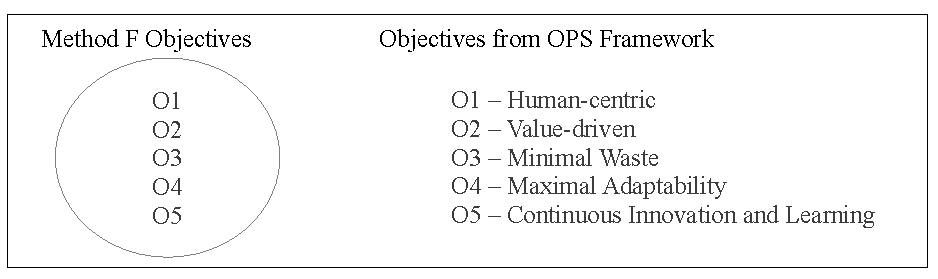
\includegraphics[scale=0.9]{include/case_study/fig/companyF_objectives.pdf}}
%\caption{Objectives identified in methodology F} 
%\label{fig:companyF_objectives}
%\end{figure}
%
%Based on the objectives and following the linkages from them, the principles were identified. As one can see in Figure~\ref{fig:companyF_objectives} methodology F does not follow the ``Frequent Reflection and Improvement" principle because the organization rarely does it re-examine the development process in order to improve it. %maybe justify why!
%It is worth mentioning that the ``Empowering teams of Motivated Individuals" principle is not entirely followed either, but it differs among the teams. Every team is built with motivated individuals, some to a more and some to a lesser extent. 
%
%\begin{figure}[H]
%\centerline{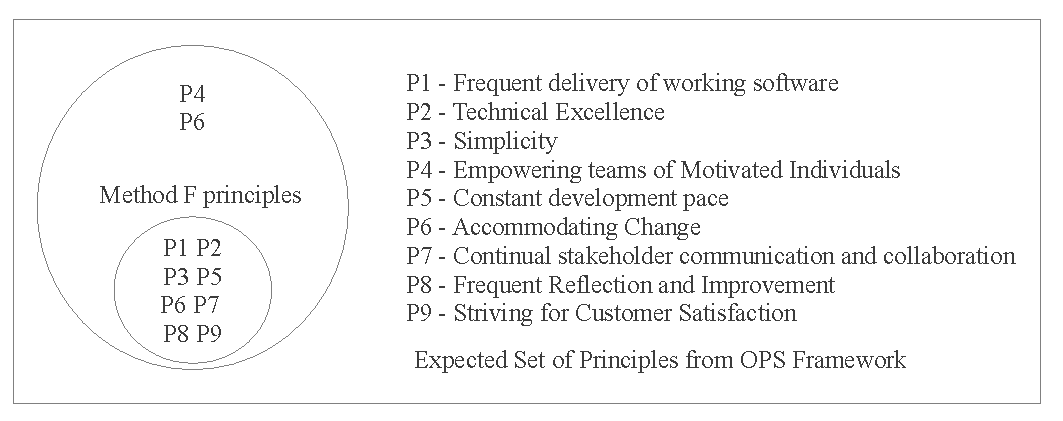
\includegraphics[scale=0.9]{include/case_study/fig/companyF_principles.pdf}}
%\caption{Principles identified in methodology F} 
%\label{fig:companyF_principles}
%\end{figure}
%
%Following the linkages from the principles the strategies for implementing them were identified. As it can be seen in Figure~\ref{fig:companyF_strategies} methodology F does not support 
%
%\begin{itemize}
%\item \textbf{Continuous feedback} - The organization does not have a defined process for getting a feedback from the customers of the company. From time to time the managers of the various departments of the company have personal conversations with the customers. If any issue arises, then they inform the development and QA departments in order to identify the problem and fix it.
%\item \textbf{Test-first development} - None of the team members writes tests before starting coding.
%\item \textbf{Constant velocity} - The organization does not measure the velocity of the teams. In general the pace of development and integration and deployment is based on the needs of the customers and the capability of the developer. No one has to finish a specific amount of work in each iteration. What is only wanted, is the functionality to be delivered when it is scheduled.
%\item \textbf{Retrospection} - Although there is a tendency to change this, the teams do not have a process for retrospection. The team members unconsciously consider that they are doing fine, unless a team leader or the manager of the department tells them the opposite.
%\end{itemize}
%
%\begin{figure}[H]
%\centerline{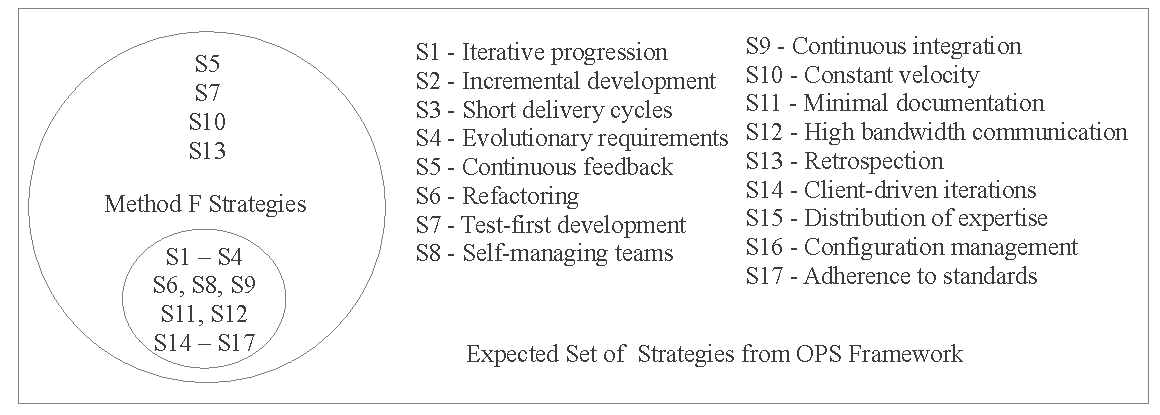
\includegraphics[scale=0.9]{include/case_study/fig/companyF_strategies.pdf}}
%\caption{Strategies identified in methodology F} 
%\label{fig:companyF_strategies}
%\end{figure}
%

%Reflecting on the above analysis, we see that methodology F lacks four strategies which are important for its improvement. Without retrospection the team members do not always identify and discuss their mistakes, while without a well defined process for continuous feedback any issues that might arise may go unnoticed for quite some time. In total, methodology F is missing four strategies out of seventeen which is a lot.

\section{Method}
\label{sec:method}

\subsection{Data Collection}

%maybe provide numbers for the demographics

%\subsubsection{Surveys}
In order to collect the data, an online survey was considered to be the best option, since it could be easily answered by each subject. In addition, this would ensure no data loss. Google Drive \texttrademark \cite{google_drive} was selected to be the platform for collecting and preserving the data.

For each of the tools, four surveys were created for each team respectively. The collection lasted about one month, the surveys for each tool were conducted every ten days. First \ac{PAM} was sent, then \ac{TAA} and at last it was \ac{OPS}.

Two subjects were requested to answer to the surveys first, in order to detect if there were any questions which could cause confusion, but also to see how much time is needed to complete a survey. Once the issues pointed out by the two subjects were fixed, the surveys were sent to the rest of the company's employees.

The links to the surveys were sent to the subjects early in the morning via email, but they were asked to reply after lunch. The reasoning for this is that at the beginning of the day the employees need to perform tasks which are usually important and time consuming, while they must have a clear head and attend meetings. On the contrary, after lunch most of the employees try to relax by enjoying their coffee and discussing with each other. That time of the day was considered to be the best in order to ask them to spend 15-20 minutes and reply to the survey. The employees that belonged to more than one teams were asked a couple of days later to take the other survey in order to verify that their answers match in both surveys. Every question of the surveys was mandatory.

As it was mentioned in chapter~\ref{ch:related_work}, \ac{PAM} focuses on the following agile practices:
\begin{inparaenum} [a\upshape)]
	\item Iteration Planning
	\item Iterative Development
	\item Continuous Integration And Testing
	\item Stand-Up Meetings
	\item Customer Access
	\item Customer Acceptance Tests
	\item Retrospectives
	\item Co-Location.
\end{inparaenum}
These showcase that methodology F does not support \textit{Stand-Up Meetings} and \textit{Retrospectives} and as a result, they were totally excluded from the surveys.

On the contrary, \ac{TAA} focuses on the following agile practices/areas:
\begin{inparaenum} [a\upshape)]
	\item Product Ownership
	\item Release Planning and Tracking
	\item Iteration Planning and Tracking
	\item Team
	\item Testing Practices
	\item Development Practices/Infrastructure.
\end{inparaenum}
From the above practices, methodology F does not support \textit{Product Ownership}, since it implies that company F should practice Scrum, which it does not. Moreover, Scrum-oriented questions from the rest of the practices/areas were removed as well. 

Finally, \ac{OPS} focuses on the following strategies:
\begin{inparaenum} [a\upshape)]
	\item Iterative progression
	\item Incremental development
	\item Short delivery cycles
	\item Evolutionary requirements
	\item Continuous feedback
	\item Refactoring
	\item Test-first development
	\item Self-managing teams
	\item Continuous integration
	\item Constant velocity
	\item Minimal documentation
	\item High bandwidth communication
	\item Retrospection
	\item Client-driven iterations
	\item Distribution of expertise
	\item Configuration management
	\item Adherence to standards

\end{inparaenum}
From the above practices, methodology F does not support \textit{Retrospection}. The company considers that meetings with the whole team do not have the desired results but rather the opposite, leading in more difficult communication and loss of time. In case a retrospection on the past events has to be held, this takes place in meeting of two or three people.
%\textit{Continuous feedback}, \textit{Constant velocity} .%(also check the analysis in section ~\ref{subsec:adequacy_analysis}

%About the questions of the agile practices/areas which were not included, they were all given a value of 1, the least possible value. 

As it was stated earlier, in subsection~\ref{subsec:ops}, \ac{OPS} agility measurements are based on three aspects: Adequacy, Capability and Effectiveness. Effectiveness measurement focuses on how well a team implements agile methodologies. Since the rest of the tools focus on the same thing, it was decided only to use the survey from Effectiveness and not to take into account the Adequacy and Capability.

For a more clear view on the questions contained in the surveys, one can take a look at Appendices~\ref{ch:effectiveness_hierarchy},~\ref{ch:pam} and~\ref{ch:team_agility_assessment}.

%\subsubsection{Likert Scales}
The surveys for \ac{PAM} \ac{TAA} and \ac{OPS} were on a Likert scale 1-7 (never-always). From \ac{PAM}, only the \textit{Co-location} practice had its Likert scale 1-5 (different time zones-same room), since its creators preferred it in this way. For the transformation of the results for this practice, the formula~\eqref{eq:likert_transformation} \cite{likert_transformation} was used.  \begin{equation} \label{eq:likert_transformation} x_2 = (1.5 * x_1) - 0.5 \end{equation} 

%\subsubsection{Demographics} % Have to fix this. Better add a table
The employees that were asked to answer to the surveys where all members of the software development teams which consisted of software and quality assurance (QA) engineers. All of the participating employees have been in the company for over a year while most of them have more than five years of work experience in an agile environment. Employees who had been working for less than six months in the company were not asked to participate, since it was considered they were not fully aware of the company's procedures or that they were not familiar enough with them. Although code review is practiced, it was avoided asking the code reviewers to take the same survey for the same team because it would not provide more value to the results and in addition, it would tire them a lot.

%\subsection{Collected Data}
Each participant replied to 176 questions in total. Initially, 34 surveys were expected to be filled in, but in the end 30 of them were filled in, since some employees preferred not to participate in the study for their own reasons.

\subsection{Data Analysis}
The data gathered from the survey were grouped on the basis of the practices covered by the \ac{OPP}, and as a consequence, the \ac{OPS}, since as one can see in Table~\ref{table:questions_coverage}, \ac{OPS} coves both \ac{PAM} and \ac{TAA}. From the 18 practices in total, four of them, \begin{inparaenum} [a\upshape)] \item Minimal or Just Enough Documentation \item Customer User Acceptance Testing \item Evolutionary Requirements \item Constant Velocity \end{inparaenum}, are covered only by one tool. The rest of the practices were covered by at least two of the tools.

Initially, there was a thought to analyse the data for each team separately, but this would create an extensive overhead. In addition, the team A has such a small number of members that the results would be inadequate to work with. As a result, it was preferred to form the data sets for each practice based on the answers from all the teams. In Table~\ref{table:data_structure}, one can see the structure of the collected data.

\begin{table} [H]
	\caption{Collected Data Structure}
	\label{table:data_structure}
	\begin{tabular}{| c | c | c | c | c |} \hline
	\textbf{Practice} & \textbf{Participants} & \textbf{\ac{PAM}} & \textbf{\ac{TAA}} & \textbf{\ac{OPS}} \\ \hline
	\multirow{3}{*}{Practice1} & Participant1 & Score1 & Score1 & Score1 \\ \hhline{~----}
	& \vdots & \vdots & \vdots  & \vdots \\ \hhline{~----}
	& ParticipantN & ScoreN & ScoreN & ScoreN \\ \hline
	\end{tabular}
\end{table}

Based on the analysis performed in Section~\ref{sec:tools_completeness}, it is clear that \ac{OPS} covers more agile practices/areas. As a result, it was decided to use these practices in order to check the correlation of the tools. In Appendix~\ref{ch:mapping}, one can see how the questions are grouped based on the \ac{OPS} practices. The data sets consist of the answers which were sorted by team as stated previously and have the same order in all practices (i.e. the nth answer in every practice is given by the same person).

For the mathematical calculations the RStudio \texttrademark \cite{rstudio} was selected since it has a wide support from its community. 

The correlation method was selected for the data analysis, as it has been used in other cases of tool comparisons \cite{jalali_angelis} \cite{Delestras2013}. The initial thought was to use ``Pearson product-moment correlation" as it is a method that is widely used in statistics. 

The four practices mentioned above were discarded for using correlation, since there would not be any.

In order to use Pearson’s correlation there must hold four prerequisites
\begin{enumerate}
\item The two variables should be measured at the interval or ratio level
\item The variables should be approximately normally distributed
\item There needs to be a linear relationship between the two variables
\item There should be no significant outliers
\end{enumerate}

Since the data were collected by surveys using Likert scales, then prerequisite \#1 is satisfied, as the Likert scales can be considered both for interval or ratio level measurements, depending on the problem each time.

As far as the normal distribution is concerned, the Shapiro-Wilk test was selected as it appears to be the most powerful normality test according to a recent paper published by \citet{Razali}. In order for a distribution to be considered normal, the p-value must be greater than the alpha level so as not to reject the null hypothesis and consider that the data are normally distributed. The chosen alpha level was 0.05 as it is the most common one.

Out of the 42 normality checks (three for each of the 14 practices), only 17 concluded that the data are normally distributed. 

The low level of normally distributed data gave a strong indication that the Pearson’s correlation would not be the appropriate way to measure the tools' correlation. As a result, it was preferred not to continue checking the last two prerequisites for Pearson’s correlation, but rather use the ``Spearman’s rank correlation coefficient" which is more adequate for non-parametric data.

In order to use Spearman’s rank correlation coefficient, two prerequisites must be satisfied
\begin{enumerate}
\item The two variables should be measured at the interval or ratio level
\item There needs to be a monotonic relationship between the two variables
\end{enumerate}

The first prerequisite has already been covered. In order to check for the monotonicity, plots were drawn between the results of each tool for all 14 practices. The plots surprisingly showed that only 8 out of 42 were monotonic, which does not allow the use of Spearman’s correlation for the rest. The Table~\ref{table:monotonic_relationships} summarizes the practices and the relationships which are monotonic and Spearman's correlation can be used. The monotonic relationships are marked in green while the non-monotonic in red.

%\begin{table} [H]
%\caption{Pairs of tools for which Spearman's correlation can be used}
%\label{table:practices_spearman}
%\begin{tabular}{| c | c |}
%\hline
%\textbf{Practice} & \textbf{Tools Correlation} \\ \hline
%Continuous Feedback & \ac{PAM} - \ac{OPS} \\ \hline
%High Bandwidth Communication & \begin{tabular}{c} \ac{PAM} - \ac{TAA} \\ \ac{PAM} - \ac{OPS} \\ \ac{TAA} - \ac{OPS} \\ \end{tabular} \\ \hline
%Client Driven Iterations &  \ac{PAM} - \ac{OPS} \\ \hline
%Continuous Integration & \ac{PAM} - \ac{TAA} \\ \hline
%Iterative and Incremental Development & \ac{PAM} - \ac{OPS} \\ \hline
%Refactoring & \ac{PAM} - \ac{TAA} \\ \hline
%\end{tabular}
%\end{table}

\begin{table}
	{\renewcommand{\arraystretch}{0.2}%
	\begin{tabular}{ | p{4cm} | p{4cm} | p{4cm} |} \hline
		\begin{tabular} { p{4cm} } 
			Adherence to Standards \\
			\begin{itemize}  \item \colorbox{red}{\ac{PAM}-\ac{TAA}} \item \colorbox{red}{\ac{PAM}-\ac{OPS}} \item \colorbox{red}{\ac{TAA}-\ac{OPS}} \end{itemize} 
		\end{tabular} &
		\begin{tabular} { p{4cm} }
			Appropriate Distribution of Expertise \\
			\begin{itemize}  \item \colorbox{red}{\ac{PAM}-\ac{TAA}} \item \colorbox{red}{\ac{PAM}-\ac{OPS}} \item \colorbox{red}{\ac{TAA}-\ac{OPS}} \end{itemize}
		\end{tabular} &
		\begin{tabular} { p{4cm} }
			Client Driven Iterations \\
			\begin{itemize}  \item \colorbox{red}{\ac{PAM}-\ac{TAA}} \item \colorbox{green}{\ac{PAM}-\ac{OPS}} \item \colorbox{red}{\ac{TAA}-\ac{OPS}} \end{itemize}
		\end{tabular} \\ \hline
		
		\begin{tabular} { p{4cm} } 
			Continuous Feedback \\
			\begin{itemize}  \item \colorbox{red}{\ac{PAM}-\ac{TAA}} \item \colorbox{green}{\ac{PAM}-\ac{OPS}} \item \colorbox{red}{\ac{TAA}-\ac{OPS}} \end{itemize}
		\end{tabular} &
		\begin{tabular} { p{4cm} }
			Continuous Integration \\
			\begin{itemize}  \item \colorbox{green}{\ac{PAM}-\ac{TAA}} \item \colorbox{red}{\ac{PAM}-\ac{OPS}} \item \colorbox{red}{\ac{TAA}-\ac{OPS}} \end{itemize}
		\end{tabular} &
		\begin{tabular} { p{4cm} }
			High Bandwidth Communication \\
			\begin{itemize}  \item \colorbox{green}{\ac{PAM}-\ac{TAA}} \item \colorbox{green}{\ac{PAM}-\ac{OPS}} \item \colorbox{green}{\ac{TAA}-\ac{OPS}} \end{itemize}
		\end{tabular} \\ \hline
		
		\begin{tabular} { p{4cm} } 
			Iteration Progress Tracking \\
			\begin{itemize}  \item \colorbox{red}{\ac{PAM}-\ac{TAA}} \item \colorbox{red}{\ac{PAM}-\ac{OPS}} \item \colorbox{red}{\ac{TAA}-\ac{OPS}} \end{itemize}
		\end{tabular} &
		\begin{tabular} { p{4cm} }
			Iterative and Incremental Development \\
			\begin{itemize}  \item \colorbox{red}{\ac{PAM}-\ac{TAA}} \item \colorbox{green}{\ac{PAM}-\ac{OPS}} \item \colorbox{red}{\ac{TAA}-\ac{OPS}} \end{itemize}
		\end{tabular} &
		\begin{tabular} { p{4cm} }
			Product Backlog \\
			\begin{itemize}  \item \colorbox{red}{\ac{PAM}-\ac{TAA}} \item \colorbox{red}{\ac{PAM}-\ac{OPS}} \item \colorbox{red}{\ac{TAA}-\ac{OPS}} \end{itemize}
		\end{tabular} \\ \hline
		
		\begin{tabular} { p{4cm} } 
			Refactoring \\
			\begin{itemize}  \item \colorbox{green}{\ac{PAM}-\ac{TAA}} \item \colorbox{red}{\ac{PAM}-\ac{OPS}} \item \colorbox{red}{\ac{TAA}-\ac{OPS}} \end{itemize}
		\end{tabular} &
		\begin{tabular} { p{4cm} }
			Self Organizing Teams \\
			\begin{itemize}  \item \colorbox{red}{\ac{PAM}-\ac{TAA}} \item \colorbox{red}{\ac{PAM}-\ac{OPS}} \item \colorbox{red}{\ac{TAA}-\ac{OPS}} \end{itemize}
		\end{tabular} &
		\begin{tabular} { p{4cm} }
			Smaller and Frequent Releases \\
			\begin{itemize}  \item \colorbox{red}{\ac{PAM}-\ac{TAA}} \item \colorbox{red}{\ac{PAM}-\ac{OPS}} \item \colorbox{red}{\ac{TAA}-\ac{OPS}} \end{itemize}
		\end{tabular} \\ \hline
		
		\begin{tabular} { p{4cm} } 
			Software Configuration Management \\
			\begin{itemize}  \item \colorbox{red}{\ac{PAM}-\ac{TAA}} \item \colorbox{red}{\ac{PAM}-\ac{OPS}} \item \colorbox{red}{\ac{TAA}-\ac{OPS}} \end{itemize}
		\end{tabular} &
		\begin{tabular} { p{4cm} }
			Test Drive Development \\
			\begin{itemize}  \item \colorbox{red}{\ac{PAM}-\ac{TAA}} \item \colorbox{red}{\ac{PAM}-\ac{OPS}} \item \colorbox{red}{\ac{TAA}-\ac{OPS}} \end{itemize}
		\end{tabular} & 
		\begin{tabular} { p{4cm} } 
			Constant Velocity \\
			\begin{itemize}  \item \colorbox{red}{\ac{PAM}-\ac{TAA}} \item \colorbox{red}{\ac{PAM}-\ac{OPS}} \item \colorbox{red}{\ac{TAA}-\ac{OPS}} \end{itemize}
		\end{tabular} \\ \hline
		
		\begin{tabular} { p{4cm} } 
			Minimal or Just Enough Documentation \\
			\begin{itemize}  \item \colorbox{red}{\ac{PAM}-\ac{TAA}} \item \colorbox{red}{\ac{PAM}-\ac{OPS}} \item \colorbox{red}{\ac{TAA}-\ac{OPS}} \end{itemize}
		\end{tabular} &
		\begin{tabular} { p{4cm} }
			Customer User Acceptance Testing \\
			\begin{itemize}  \item \colorbox{red}{\ac{PAM}-\ac{TAA}} \item \colorbox{red}{\ac{PAM}-\ac{OPS}} \item \colorbox{red}{\ac{TAA}-\ac{OPS}} \end{itemize}
		\end{tabular} &
		\begin{tabular} { p{4cm} }
			Evolutionary Requirements \\
			\begin{itemize}  \item \colorbox{red}{\ac{PAM}-\ac{TAA}} \item \colorbox{red}{\ac{PAM}-\ac{OPS}} \item \colorbox{red}{\ac{TAA}-\ac{OPS}} \end{itemize}
		\end{tabular} \\ \hline
	\end{tabular}}
	\caption{Monotonic Relationships}
	\label{table:monotonic_relationships}	
\end{table}



\section{Threats to Validity}
\textbf{Note to Lucas}
I will continue for the rest of the study, but this should be a separate chapter. Or should I have one after each thematic subject? (i.e. tools completeness, case study, \ac{OPS} enhancement)

\bigskip

Validity threats exist in every case study and this one could not be an exception.

\subsection{Construct Validity}
Construct validity mainly deals with obtaining the right method for the concept under study \cite{Wohlin}.

Structural?
Convergent validity?

\subsection{Internal Validity}
Internal validity deals with the issues that may affect the casual relationship between treatment and results \cite{Wohlin}. The creators of \ac{PAM}, \ac{TAA} and \ac{OPS} have already tried to mitigate this when creating their tools. Yet, there are still some aspects of internal validity, such as selection bias and maturation. As far as maturation is concerned, this comes to boredom on the responses given by the teams. Although the surveys were small in size and did not require more than 15-20 minutes each, still the possibly repetitive questions on the topic could cause boredom to the subjects. The mitigation for this threat was to separate the surveys in three different weeks. In addition, the respondents could stop the survey at any point and continue whenever they wanted. Finally, selection could not be mitigated as a threat since the case study focused on a specific company.

\subsection{Conclusion Validity}
Conclusion validity concerns the possibility of reaching a wrong conclusion \cite{Wohlin}. Although the questions of the surveys have been carefully created, still there may be uncertainty about them. In order to mitigate this, for each survey a pilot one was conducted to spot any misunderstandings. In addition, the participants could ask the author of this thesis for any questions they had concerning the survey questions.

\subsection{External Validity}
External validity deals with the ability to generalize the outcomes of the case study \cite{Wohlin}. Every software development team, even in the same company, applies agile methodologies in different ways. Nevertheless, the correlations among the tools are not context-specific and should not differ a lot due to the reasons explained in section~\ref{sec:findings}. Yet, as it is known, conducting a case study is susceptible to generalizing its outcomes. In this case though, we can consider that teams following the same agile practices should not have different results.


\section{Correlation Results}
The cells for which a correlation exists are coloured in green in order to distinguish them from the rest. In Table~\ref{table:correlations_frequency} one can see that half of the correlations are between \ac{PAM} and \ac{OPS}. This corroborates that \ac{OPS} has full coverage of \ac{PAM} as seen in Table ~\ref{table:questions_coverage}. %maybe add in the Analysis - chapter 4

\begin{table} [H]
 \RawFloats %allows to have captions in all of the tables
 \begin{minipage}{.45\textwidth}
  \caption{Continuous Feedback Correlations}
  \label{table:cf_correlations}
   \begin{tabular}{| c | c | c | c |} \hline
   \multicolumn{4}{|c|}{\textbf{Continuous Feedback}}  \\ \hline
   & \ac{PAM} & \ac{TAA} & \ac{OPS} \\ \hline
   \ac{PAM} & 1.000 & NA & \cellcolor{green}0.459 \\ \hline
   \ac{TAA} & NA & 1.000 & NA \\ \hline
   \ac{OPS} & \cellcolor{green}0.459 & NA & 1.000 \\ \hline
  \end{tabular}
 \end{minipage}%
%
 \begin{minipage}{.45\textwidth}
  \centering
  \caption{Client Driven Iterations Correlations}
  \label{table:cdi_correlations}
  \begin{tabular}{| c | c | c | c |} \hline
  \multicolumn{4}{|c|}{\textbf{Client Driven Iterations}}  \\ \hline
   & \ac{PAM} & \ac{TAA} & \ac{OPS} \\ \hline
  \ac{PAM} & 1.000 & NA & \cellcolor{green}0.161 \\ \hline
  \ac{TAA} & NA & 1.000 & NA \\ \hline
  \ac{OPS} & \cellcolor{green}0.161 & NA & 1.000 \\ \hline
 \end{tabular}
 \end{minipage}%
 %
\end{table}


\begin{table} [H]
 \RawFloats %allows to have captions in all of the tables
 \begin{minipage}{.45\textwidth}
  \caption{High Bandwidth Communication Correlations}
  \label{table:hbc_correlations}
  \begin{tabular}{| c | c | c | c |} \hline
  \multicolumn{4}{|c|}{\textbf{High Bandwidth Communication}}  \\ \hline
  & \ac{PAM} & \ac{TAA} & \ac{OPS} \\ \hline
  \ac{PAM} & 1.000 & \cellcolor{green}0.322 & \cellcolor{green}-0.023 \\ \hline
  \ac{TAA} & \cellcolor{green}0.322 & 1.000 & \cellcolor{green}0.237 \\ \hline
  \ac{OPS} & \cellcolor{green}-0.023 & \cellcolor{green}0.237 & 1.000 \\ \hline
 \end{tabular}
 \end{minipage}%
%
 \begin{minipage}{.45\textwidth}
  \centering
  \caption{Refactoring Correlations}
  \label{table:ref_correlations}
  \begin{tabular}{| c | c | c | c |} \hline
  \multicolumn{4}{|c|}{\textbf{Refactoring}}  \\ \hline
   & \ac{PAM} & \ac{TAA} & \ac{OPS} \\ \hline
   \ac{PAM} & 1.000 & \cellcolor{green}0.097 & -0.050 \\ \hline
   \ac{TAA} & \cellcolor{green}0.097 & 1.000 & 0.181 \\ \hline
   \ac{OPS} & -0.050 & 0.181 & 1.000 \\ \hline
  \end{tabular}  
 \end{minipage}%
 %
\end{table}

\begin{table} [H]
 \RawFloats %allows to have captions in all of the tables
 \begin{minipage}{.45\textwidth}
  \caption{Continuous Integration Correlations}
  \label{table:ci_correlations}
  \begin{tabular}{| c | c | c | c | } \hline
  \multicolumn{4}{|c|}{\textbf{Continuous Integration}}  \\ \hline
   & \ac{PAM} & \ac{TAA} & \ac{OPS} \\ \hline
  \ac{PAM} & 1.000 & 0.398 & \cellcolor{green}0.249 \\ \hline
  \ac{TAA} & 0.398 & 1.000 & 0.115 \\ \hline
  \ac{OPS} & \cellcolor{green}0.249 & 0.115 & 1.000 \\ \hline
 \end{tabular}
 \end{minipage}%
%
 \begin{minipage}{.45\textwidth}
  \centering
   \caption{Iterative and Incremental Development Correlations}
  \label{table:iid_correlations}
  \begin{tabular}{| c | c | c | c |} \hline
  \multicolumn{4}{|c|}{\textbf{Iterative and Incremental Development}}  \\ \hline
  & \ac{PAM} & \ac{TAA} & \ac{OPS} \\ \hline
  \ac{PAM} & 1.000 & 0.204 & \cellcolor{green}0.396 \\ \hline
  \ac{TAA} & 0.204 & 1.000 & -0.228 \\ \hline
  \ac{OPS} & \cellcolor{green}0.396 & -0.228 & 1.000 \\ \hline
 \end{tabular}
 \end{minipage}%
 %
\end{table}

\begin{table} [H]
	\caption{Frequency of correlation between tools}
	\label{table:correlations_frequency}
	\begin{tabular}{| c | c |} \hline
		\multicolumn{2}{|c|}{\textbf{Frequency}}  \\ \hline
		\ac{PAM}-\ac{OPS} & 4 \\ \hline
		\ac{PAM}-\ac{TAA} & 3 \\ \hline
		\ac{TAA}-\ac{OPS} & 1 \\ \hline
	\end{tabular}
\end{table}


In Table~\ref{table:descriptive_statistics} one can see the descriptive statistics of the data gathered.

	\begin{longtable}{| p{.13\textwidth} | p{.11\textwidth} | p{.06\textwidth} | p{.06\textwidth} | p{.06\textwidth} | p{.13\textwidth} | p{.11\textwidth} | p{.06\textwidth} | p{.06\textwidth} | p{.06\textwidth} |} \caption{Descriptive Statistics} \\ \hline 
		\label{table:descriptive_statistics}
		\textbf{Practice} & \textbf{Statistics} & \textbf{\ac{PAM}} & \textbf{\ac{TAA}} & \textbf{\ac{OPS}} &
		\textbf{Practice} & \textbf{Statistics} & \textbf{\ac{PAM}} & \textbf{\ac{TAA}} & \textbf{\ac{OPS}} \\ \hline
		\endhead %repeats the header to the next page
		Adherence to Standards & \begin{tabular}{c} Mean \\ Sd \\ Median \\ Min \\ Max \end{tabular} & 
		\begin{tabular}{c} 1.00 \\ 0.00 \\ 1 \\ 1 \\ 1 \end{tabular} & 
		\begin{tabular}{c} 11.67 \\ 2.17 \\ 12 \\ 7 \\ 14 \end{tabular} & 
		\begin{tabular}{c} 8.10 \\ 2.12 \\ 8 \\ 6 \\ 12 \end{tabular} &	
		Appropriate Distribution of Expertise & \begin{tabular}{c} Mean \\ Sd \\ Median \\ Min \\ Max \end{tabular} &
		\begin{tabular}{c} 1.00 \\ 0.00 \\ 1.0 \\ 1 \\ 1 \end{tabular} & 
		\begin{tabular}{c} 11.13 \\ 2.10 \\ 11.5 \\ 6 \\ 14 \end{tabular} & 
		\begin{tabular}{c} 27.20 \\ 3.51 \\ 27.0 \\ 21 \\ 35 \end{tabular} \\ \hline		
		Client-Driven Iterations & \begin{tabular}{c} Mean \\ Sd \\ Median \\ Min \\ Max \end{tabular} &
		\begin{tabular}{c} 8.63 \\ 3.20 \\ 8.5 \\ 3 \\ 14 \end{tabular} & 
		\begin{tabular}{c} 1.00 \\ 0.00 \\ 1.0 \\ 1 \\ 1 \end{tabular} & 
		\begin{tabular}{c} 13.87 \\ 2.78 \\ 14.0 \\ 9 \\ 21 \end{tabular} &	
		Continuous Feedback & \begin{tabular}{c} Mean \\ Sd \\ Median \\ Min \\ Max \end{tabular} &
		\begin{tabular}{c} 4.87 \\ 1.25 \\ 5.0 \\ 2 \\ 7 \end{tabular} & 
		\begin{tabular}{c} 1.00 \\ 0.00 \\ 1.0 \\ 1 \\ 1 \end{tabular} & 
		\begin{tabular}{c} 9.20 \\ 1.88 \\ 9.5 \\ 5 \\ 14 \end{tabular} \\ \hline		
		Continuous Integration & \begin{tabular}{c} Mean \\ Sd \\ Median \\ Min \\ Max \end{tabular} &
		\begin{tabular}{c} 21.97 \\ 4.40 \\ 21.0 \\ 11 \\ 31 \end{tabular} & 
		\begin{tabular}{c} 24.13 \\ 3.82 \\ 24.5 \\ 16 \\ 31 \end{tabular} & 
		\begin{tabular}{c} 48.10 \\ 4.23 \\ 48.5 \\ 40 \\ 56 \end{tabular} &	
		High-Bandwidth Communication & \begin{tabular}{c} Mean \\ Sd \\ Median \\ Min \\ Max \end{tabular} &
		\begin{tabular}{c} 36.73 \\ 4.11 \\ 38 \\ 29 \\ 42 \end{tabular} & 
		\begin{tabular}{c} 22.87 \\ 3.25 \\ 23 \\ 13 \\ 28 \end{tabular} & 
		\begin{tabular}{c} 60.30 \\ 5.69 \\ 60 \\ 51 \\ 75 \end{tabular} \\ \hline		
		Iteration Progress Tracking and Reporting & \begin{tabular}{c} Mean \\ Sd \\ Median \\ Min \\ Max \end{tabular} &
		\begin{tabular}{c} 21.67 \\ 6.42 \\ 22.5 \\ 8 \\ 35 \end{tabular} & 
		\begin{tabular}{c} 71.73 \\ 15.62 \\ 72.5 \\ 40 \\ 100 \end{tabular} & 
		\begin{tabular}{c} 31.73 \\ 1.55 \\ 32.0 \\ 27 \\ 35 \end{tabular} &	
		Iterative and Incremental Development & \begin{tabular}{c} Mean \\ Sd \\ Median \\ Min \\ Max \end{tabular} &
		\begin{tabular}{c} 27.10 \\ 2.71 \\ 27.0 \\ 22 \\ 34 \end{tabular} &
		\begin{tabular}{c} 8.43 \\ 2.11 \\ 8.5 \\ 4 \\ 13 \end{tabular} &
		\begin{tabular}{c} 14.47 \\ 2.13 \\ 15.0 \\ 11 \\ 18 \end{tabular} \\ \hline		
		Product Backlog & \begin{tabular}{c} Mean \\ Sd \\ Median \\ Min \\ Max \end{tabular} &
		\begin{tabular}{c} 1.00 \\ 0.00 \\ 1.0 \\ 1 \\ 1 \end{tabular} &
		\begin{tabular}{c} 4.97 \\ 0.85 \\ 5.0 \\ 3 \\ 6 \end{tabular} &
		\begin{tabular}{c} 15.80 \\ 2.14 \\ 15.5 \\ 12 \\ 19 \end{tabular}  &
		Refactoring & \begin{tabular}{c} Mean \\ Sd \\ Median \\ Min \\ Max \end{tabular} &
		\begin{tabular}{c} 2.03 \\ 0.85 \\ 2.0 \\ 1 \\ 4 \end{tabular} &
		\begin{tabular}{c} 10.80 \\ 2.27 \\ 11.0 \\ 6 \\ 14 \end{tabular} &
		\begin{tabular}{c} 20.67 \\ 3.66 \\ 20.5 \\ 14 \\ 28 \end{tabular}  \\ \hline
		Self-Organizing Teams & \begin{tabular}{c} Mean \\ Sd \\ Median \\ Min \\ Max \end{tabular} &
		\begin{tabular}{c} 3.6 \\ 1.19 \\ 3.5 \\ 2 \\ 6 \end{tabular} &
		\begin{tabular}{c} 62.9 \\ 6.57 \\ 63.0 \\ 48 \\ 75 \end{tabular} &
		\begin{tabular}{c} 36.5 \\ 5.20 \\ 37.0 \\ 26 \\ 45 \end{tabular}  &
		Smaller and Frequent Product Releases & \begin{tabular}{c} Mean \\ Sd \\ Median \\ Min \\ Max \end{tabular} &
		\begin{tabular}{c} 5.6 \\ 1.19 \\ 6 \\ 2 \\ 7 \end{tabular} &
		\begin{tabular}{c} 5.8 \\ 0.81 \\ 6 \\ 4 \\ 7 \end{tabular} &
		\begin{tabular}{c} 24.8 \\ 1.24 \\ 25 \\ 22 \\ 28 \end{tabular} \\ \hline		
		Software Configuration Management & \begin{tabular}{c} Mean \\ Sd \\ Median \\ Min \\ Max \end{tabular} &
		\begin{tabular}{c} 1 \\ 0 \\ 1 \\ 1 \\ 1 \end{tabular} &
		\begin{tabular}{c} 7 \\ 0 \\ 7 \\ 7 \\ 7 \end{tabular} &
		\begin{tabular}{c} 7 \\ 0 \\ 7 \\ 7 \\ 7 \end{tabular} &
		Test Driven Development & \begin{tabular}{c} Mean \\ Sd \\ Median \\ Min \\ Max \end{tabular} &
		\begin{tabular}{c} 10.90 \\ 2.90 \\ 10.5 \\ 6 \\ 17 \end{tabular} &
		\begin{tabular}{c} 6.57 \\ 3.28 \\ 6.0 \\ 3 \\ 15 \end{tabular} &
		\begin{tabular}{c} 9.10 \\ 1.97 \\ 9.0 \\ 6 \\ 13 \end{tabular} \\ \hline
		Minimal or Just Enough Documentation & \begin{tabular}{c} Mean \\ Sd \\ Median \\ Min \\ Max \end{tabular} &
		\begin{tabular}{c} 1.0 \\ 0.00 \\ 1 \\ 1 \\ 1 \end{tabular} &
		\begin{tabular}{c} 1.0 \\ 0.00 \\ 1 \\ 1 \\ 1 \end{tabular} &
		\begin{tabular}{c} 17.8 \\ 3.16 \\ 18 \\ 10 \\ 23 \end{tabular} &	
		Customer User Acceptance Testing & \begin{tabular}{c} Mean \\ Sd \\ Median \\ Min \\ Max \end{tabular} &
		\begin{tabular}{c} 17.37 \\ 7.04 \\ 17.5 \\ 5 \\ 33 \end{tabular} &
		\begin{tabular}{c} 1.00 \\ 0.00 \\ 1.0 \\ 1 \\ 1 \end{tabular} &
		\begin{tabular}{c} 1.00 \\ 0.00 \\ 1.0 \\ 1 \\ 1 \end{tabular} \\ \hline
		Evolutionary Requirements & \begin{tabular}{c} Mean \\ Sd \\ Median \\ Min \\ Max \end{tabular} &
		\begin{tabular}{c} 1.00 \\ 0.00 \\ 1 \\ 1 \\ 1 \end{tabular} &
		\begin{tabular}{c} 1.00 \\ 0.00 \\ 1 \\ 1 \\ 1 \end{tabular} &
		\begin{tabular}{c} 20.13 \\ 2.21 \\ 20 \\ 17 \\ 25 \end{tabular} &
		Constant Velocity & \begin{tabular}{c} Mean \\ Sd \\ Median \\ Min \\ Max \end{tabular} &
		\begin{tabular}{c} 1.00 \\ 0.00 \\ 1 \\ 1 \\ 1 \end{tabular} &
		\begin{tabular}{c} 5.93 \\ 1.01 \\ 6 \\ 4 \\ 7 \end{tabular} &
		\begin{tabular}{c} 1.00 \\ 0.00 \\ 1 \\ 1 \\ 1 \end{tabular} \\ \hline
\end{longtable}


%\section{Analysis}
%\label{sec:analysis}
%
%\subsection{Introduction}
%As it has already been presented, the correlation of only a few of the practices can be examined. In this section the reasons that did not allow the calculation of the correlation will be presented and discussed.

%\section{Correlations Analysis}
%\label{subsec:correlation_analysis}

In \textit{Continuous Feedback} \ac{PAM} and \ac{OPS} have a moderate positive correlation of $\rho$ = 0.459. Both tools focus on getting feedback from the customer, while \ac{OPS} also checks whether the product is developed according to the customer's needs and expectations.

In \textit{Client-Driven Iterations} \ac{PAM} and \ac{OPS} have a low positive correlation of $\rho$ = 0.161. Both tools check for the possibility of the requirements having been prioritized by the customer. Moreover, the \ac{OPS} focuses on the customers' requests and needs.

In \textit{Continuous Integration} \ac{PAM} and \ac{OPS} have a low positive correlation of $\rho$ = 0.249. The common areas are continuous builds, multiple submits and story acceptance. There is a small difference regarding whether the developers should sync to the latest available code that is supported by the \ac{PAM}.

\textit{Iterative and Incremental Development} \ac{PAM} and \ac{OPS} have a low positive correlation of $\rho$ = 0.396. The \ac{OPS} focuses on the stories estimation and prioritization, while \ac{PAM} on the deadlines that have to be meet and on the software progress. 

\textit{High Bandwidth Communication} \ac{PAM} and \ac{TAA} have a low positive correlation of $\rho$ = 0.322. Both of them check for the team co-location, while \ac{TAA} also checks for the communication with the customers. \ac{PAM} and \ac{OPS} have correlation of $\rho$ = -0.023 which means there is no correlation at all. They both focus on the communication, but \ac{OPS} does that to a huge extent, resulting in such an extremely low correlation. In addition, \ac{OPS} checks for effectively using the time for meetings. \ac{TAA} and \ac{OPS} have a positive correlation of $\rho$ = 0.237. This is the only practice for which correlation exists for all the tools.

\textit{Refactoring} \ac{PAM} and \ac{TAA} have a correlation of $\rho$ = 0.097, which means there is almost no correlation at all. \ac{TAA} focuses on continuous refactoring, while on the other hand \ac{PAM} on unit testing.


\section{Findings}
\label{sec:findings}

The plots showed a quite interesting result. Not only don’t the tools have a correlation, but they do not have a monotonic relationship either between one another for the agile practices covered (see Table~\ref{table:monotonic_relationships}). The absence of monotonicity shows that the questions used by the tools in order to cover an agile practice, do it differently and that \ac{PAM}, \ac{TAA} and \ac{OPS} measure the agility of software development teams in their own unique way. Each of the tools was constructed and validated by its creators having the agile concept in mind, but apparently following a different path in order to accomplish it. This is quite clear by looking on the different ways that each practice is covered (see Appendix~\ref{ch:mapping}) where many of the questions have a different perspective on measuring a practice although they focus on the same one. The reasons for this unexpected phenomenon are explained in the next paragraphs.

\subsection{The tools measure a practice in the same way}
Tools that claim to measure agility in the same way are expected to do so. Unfortunately, this does not imply that their correlation can be calculated. The figure~\ref{fig:scm_plot} made it very clear why. All the answers from all the teams and for \ac{TAA} and \ac{OPS} were the same. Both tools had a unique question about using a version control management system, which holds for the company F over anything that has to do with code changes. The designed plots only had one spot which means that the correlation among the tools is not possible to calculate due to the lack of variation in the results. Such an occurrence shows that correlation techniques can be defective when checking tools which manage to measure the same thing to the same extent.

\subsection{The tools have few or no questions for measuring a practice}
Another reason for not being able to calculate the correlation of the tools is that they cover slightly or even not at all some of the practices. An example of this is the \textit{Smaller and Frequent Product Releases} practice. \ac{OPS} has four questions for it, while on the other hand, \ac{PAM} and \ac{TAA} have a single one each. Furthermore, \textit{Appropriate Distribution of Expertise} is not covered at all by \ac{PAM} while it is by the rest of the tools. In case the single question gets a low score, this will affect the effectiveness of the tool. On the contrary, multiple questions can cover the practice more completely by examining more factors that affect it. Apart from measuring a practice more precisely, this also has the benefit that even if one question gets a low score, the rest of them are candidates for getting a higher one. The issue is worse if a practice is not covered at all. Unfortunately, this phenomenon does not allow to equally check all the tools, since it is giving a superiority to the ones that take the practice into consideration and even more to the ones that do that to an extensive degree.

\subsection{The tools measure the same practice differently}
Something very interesting that came up during the data analysis was that although the tools cover the same practices, they do it in different ways, leading to different results. An example of this is the practice of \textit{Refactoring} ~\ref{fig:ref_plot}. \ac{PAM} checks whether there are enough unit tests and automated system tests to allow the safe code refactoring. In case that the course unit/system tests are not developed by a team, the respondents will give low scores to the question, as the team members in company F did. Nevertheless, this does not mean that the team never refactors the software or it does it with bad results. All teams in company F choose to refactor when it adds value to the system, but the level of unit tests is very low and they exist only for specific teams. On the other hand, \ac{TAA} and \ac{OPS} check how often the teams refactor among other factors, which allows to better evaluate the practice of refactoring. Considering the above, \ac{PAM} seems to fail measuring the \textit{Refactoring}.

\subsection{The tools measure the same practice in opposite questions}
\label{subsec:opposite_questions}
The \textit{Continuous Integration} practice has a unique paradox among \ac{TAA}, \ac{PAM} and \ac{OPS}. The first two tools have a question about the members of the team having synced to the latest code, while \ac{OPS} checks for the exact opposite. According to \citet{sventha_dissertation}, it is preferable for the teams not to share the same code in order to measure the practice. It is quite doubtful though how correct this question can be, since the \textit{Continuous Integration} requires frequent submits from the developers and thus the rest of the team will also have a local version of the code.

\subsection{Questions phrasing}
Although the tools might cover the same areas for each practice, the results could differ because of how a question is structured. An example of this is the \textit{Test Driven Development} practice. Both \ac{TAA} and \ac{PAM} ask about automated code coverage, while \ac{OPS} just asks about the existence of code coverage. Furthermore, \ac{TAA} focuses on 100\% automation while \ac{PAM} doesn’t. Thus, if a team has code coverage but it is not automated, then the score of the respective question should be low. In case of \ac{TAA}, if it is fully automated, it should be even lower. It is evident that the more specific a question is, the more its answer will differ, resulting in possible low scores.

\subsection{How people perceive agility --- Maybe add this at the final discussion of the document?}
Although the concept of agility is not new, people do not seem to fully understand it. This is actually the reason for having so many tools in the field trying to measure how agile the teams are or the methodologies used. Teams implement agile methodologies differently and researchers create different measurement tools. There are numerous definitions about what agility is \cite{Kidd, NagelDove, Kara, Ramesh}, and each of the tools creator adopt or adapt the tools to match their needs. Their only common basis is the agile manifesto \cite{beck2001agile} and its twelve principles \cite{agile_principles}, which are (and should be considered as) a compass for the agile practitioners. Nevertheless, they are not enough and this resulted in the saturation of the field. Moreover, \citet{conboy_fitzgerald} state that the Agile Manifesto principles do not provide practical understanding of the concept of Agility. Consequently, all the reasons behind the current survey results are driven by the way in which people perceive agility. The word ``people" refers to the tool creators and tool users.

The questions in the surveys were all based on how their creators perceived the agile concept which is quite vague. As the reader has seen in previous chapters, \ac{PAM}, \ac{TAA} and \ac{OPS} focus on some common areas/practices, such as  \textit{Smaller and Frequent Product Releases} and \textit{High-Bandwidth Communication}, while many are different. None of the \citet{sventha_dissertation}, \citet{pam}, \citet{Leffingwell} claimed of course to have created the most complete measurement tool, but still this leads to the oxymoron that the tools created by specialists to measure the agility of software development tools, actually do it differently without providing substantial solution to the problem. On the contrary, this leads to more confusion for the agile practitioners who are at a loose ends.

Considering that the researchers and specialists in the agile field perceive the concept of agility differently, it would be naive to say that the teams do not do the same. The answers in surveys are subjective and people answer them depending on how they understand them. This is also corroborated by the fact that although a team works at the same room and follows the same processes for weeks, it is rather unlikely if its members to have the same understanding of what a retrospection or a releasing planning meeting means for them.

\section{Agile Practices Correlations}
Regarding RQ \#2, \textit{``In what ways do the tools correlate"}, it was seen that the agile practices correlations almost do not exist at all between \ac{PAM}, \ac{TAA} and \ac{OPS}. Only 8 our 42 relationships have a correlation and they are mostly positive but low.

\section{Chapter Summary}
In this chapter was presented how much complete were the tools among them. \ac{OPS} covers both \ac{PAM} and \ac{TAA} to a bug extent. In the second part the case study took place which showed that only 8 out of 42 relationships between the agile practices do correlate. The rest lack monotonicity due to
\begin{inparaenum} [a\upshape)]
	\item measuring a practice in the same way,
	\item having few or no questions for measuring a practice,
	\item measuring the same practice differently,
	\item measuring the same practice in opposite questions,
	\item questions phrasing
\end{inparaenum}

%\begin{longtable}{| p{.10\textwidth} | p{.12\textwidth} | p{.09\textwidth} | p{.09\textwidth} | p{.09\textwidth} | p{.09\textwidth} | p{.09\textwidth} |}  \hline
%	\textbf{Practice} & \textbf{Tools} & \textbf{Mean} & \textbf{Sd} & \textbf{Median} & \textbf{Min} & \textbf{Max} \\ \hline
%	Adherence to Standards & \begin{tabular}{c} \ac{PAM} \\ \ac{TAA} \\ \ac{OPS} \end{tabular} & 
%	\begin{tabular}{c} 1.00 \\ 11.67 \\ 8.10	\end{tabular} & \begin{tabular}{c} 0 \\ 2.17 \\ 2.12 	\end{tabular} & \begin{tabular}{c} 1 \\ 12 \\ 8	\end{tabular} & \begin{tabular}{c} 1 \\ 7 \\ 6 \end{tabular} & \begin{tabular}{c} 1 \\ 14 \\ 12 \end{tabular} \\ \hline
%\end{longtable}


%FIX VALUES FOR \ac{PAM}
%
%In the Tables~\ref{table:pam_results} and~\ref{table:taa_results} one can see the average value of the team replies in every agile practice/area \footnote{The ones  marked with $^\ast$ are not included in the surveys}. All the answers were trimmed to two decimal points.
%
%\begin{table} [H]
%\caption{Perceptive Agile Measurement Results}
%\label{table:pam_results}
%\begin{tabular}{| c | c | c | c | c |}
%\hline
%  & \multicolumn{4}{c|}{\textbf{Team}} \\ \hline
%\textbf{Practice} & Mobile & Info & POS & Marketing \\ \hline
%Iteration Planning & 3.86 & 5 & 4.08 & 3.66 \\ \hline
%Iterative Development & 4.36 & 5.71 & 5.3 & 5.09 \\ \hline
%Continuous Integration And Testing & 4.28 & 3.7 & 4.29 & 4.2 \\ \hline
%Customer Access & 4.58 & 7 & 5.5 & 3.9 \\ \hline
%Customer Acceptance Tests & 3.4 & 3.4 & 3.83 & 1.64 \\ \hline
%Co-Location & 4.27 & 6.13 & 5.59 & 6.2 \\ \hline 
%Stand-Up Meetings$^\ast$ & 1 & 1 & 1 & 1 \\ \hline
%Retrospectives$^\ast$ & 1 & 1 & 1 & 1 \\ \hline
%\textbf{Total} & 3.47 & 4.12 & 3.82 & 3.53 \\ \hline
%\end{tabular}
%\end{table}
%
%\begin{table} [H]
%\caption{Team Agility Assessment Results}
%\label{table:taa_results}
%\begin{tabular}{| c | c | c | c | c |}
%\hline
%  & \multicolumn{4}{c|}{\textbf{Team}} \\ \hline
%\textbf{Agile Area} & Mobile & Info & POS & Marketing \\ \hline
%Release Planning and Tracking & 4.54 & 4.17 & 4.43 & 4.38 \\ \hline
%Iteration Planning and Tracking & 3.98 & 3.58 & 4.04 & 3.7 \\ \hline
%Team & 4.95 & 4.93 & 4.73 & 4.44 \\ \hline
%Testing Practices & 3.86 & 2.56 & 3.3 & 3.77 \\ \hline
%Development Practices/Infrastructure & 5.92 & 5.94 & 5.49 & 5.5 \\ \hline
%Product Ownership$^\ast$ & 1 & 1 & 1 & 1 \\ \hline 
%\textbf{Total} & 4.04 & 3.7 & 3.83 & 3.8 \\ \hline
%\end{tabular}
%\end{table}